% Created by tikzDevice version 0.12 on 2019-03-01 10:09:53
% !TEX encoding = UTF-8 Unicode
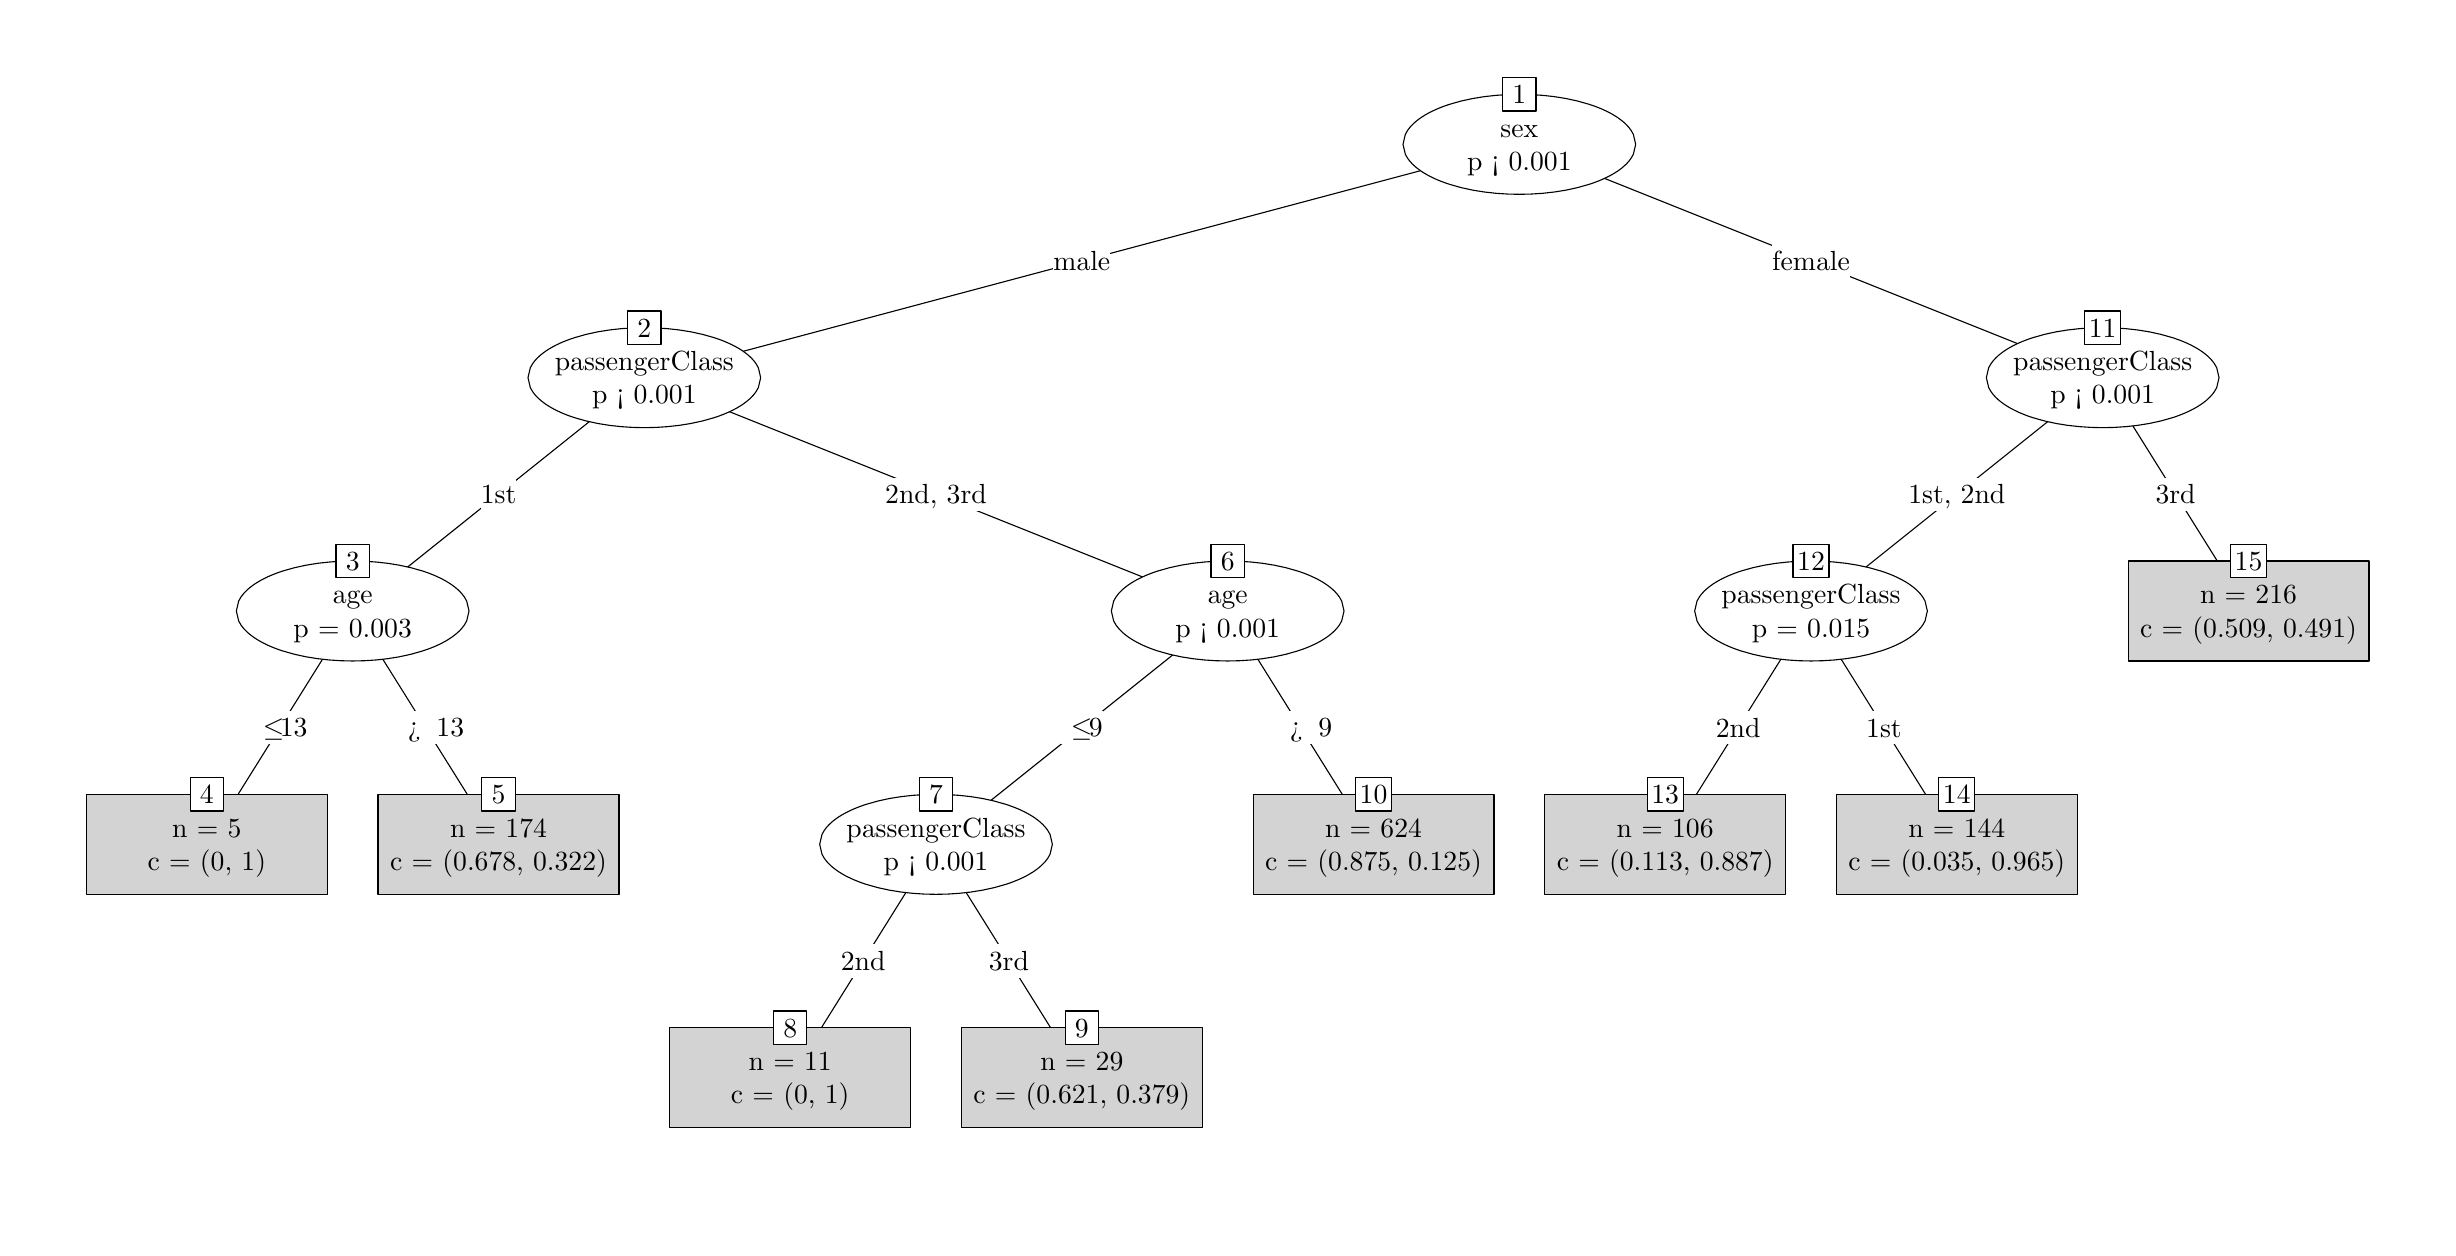
\begin{tikzpicture}[x=1pt,y=1pt]
\definecolor{fillColor}{RGB}{255,255,255}
\path[use as bounding box,fill=fillColor,fill opacity=0.00] (0,0) rectangle (867.24,433.62);
\begin{scope}
\path[clip] (  0.00,  0.00) rectangle (867.24,433.62);
\definecolor{drawColor}{RGB}{0,0,0}

\path[draw=drawColor,line width= 0.4pt,line join=round,line cap=round] (539.01,391.46) --
	(222.83,307.15);

\path[draw=drawColor,line width= 0.4pt,line join=round,line cap=round] (539.01,391.46) --
	(749.80,307.15);
\definecolor{fillColor}{RGB}{255,255,255}

\path[draw=drawColor,line width= 0.4pt,line join=round,line cap=round,fill=fillColor] (496.97,391.46) --
	(497.81,395.06) --
	(498.65,396.52) --
	(499.50,397.63) --
	(500.34,398.54) --
	(501.18,399.34) --
	(502.02,400.04) --
	(502.86,400.68) --
	(503.70,401.27) --
	(504.54,401.80) --
	(505.38,402.30) --
	(506.22,402.77) --
	(507.06,403.20) --
	(507.90,403.61) --
	(508.74,404.00) --
	(509.58,404.37) --
	(510.43,404.71) --
	(511.27,405.04) --
	(512.11,405.35) --
	(512.95,405.64) --
	(513.79,405.92) --
	(513.79,405.92) --
	(517.99,407.11) --
	(522.20,408.02) --
	(526.40,408.70) --
	(530.61,409.16) --
	(534.81,409.44) --
	(539.01,409.53) --
	(543.22,409.44) --
	(547.42,409.16) --
	(551.63,408.70) --
	(555.83,408.02) --
	(560.03,407.11) --
	(564.24,405.92) --
	(564.24,405.92) --
	(565.08,405.64) --
	(565.92,405.35) --
	(566.76,405.04) --
	(567.60,404.71) --
	(568.44,404.37) --
	(569.28,404.00) --
	(570.12,403.61) --
	(570.97,403.20) --
	(571.81,402.77) --
	(572.65,402.30) --
	(573.49,401.80) --
	(574.33,401.27) --
	(575.17,400.68) --
	(576.01,400.04) --
	(576.85,399.34) --
	(577.69,398.54) --
	(578.53,397.63) --
	(579.37,396.52) --
	(580.21,395.06) --
	(581.05,391.46) --
	(581.05,391.46) --
	(580.21,387.87) --
	(579.37,386.40) --
	(578.53,385.30) --
	(577.69,384.38) --
	(576.85,383.59) --
	(576.01,382.88) --
	(575.17,382.24) --
	(574.33,381.66) --
	(573.49,381.12) --
	(572.65,380.62) --
	(571.81,380.16) --
	(570.97,379.72) --
	(570.12,379.31) --
	(569.28,378.92) --
	(568.44,378.56) --
	(567.60,378.22) --
	(566.76,377.89) --
	(565.92,377.58) --
	(565.08,377.29) --
	(564.24,377.01) --
	(564.24,377.01) --
	(560.03,375.82) --
	(555.83,374.90) --
	(551.63,374.23) --
	(547.42,373.76) --
	(543.22,373.49) --
	(539.01,373.40) --
	(534.81,373.49) --
	(530.61,373.76) --
	(526.40,374.23) --
	(522.20,374.90) --
	(517.99,375.82) --
	(513.79,377.01) --
	(513.79,377.01) --
	(512.95,377.29) --
	(512.11,377.58) --
	(511.27,377.89) --
	(510.43,378.22) --
	(509.58,378.56) --
	(508.74,378.92) --
	(507.90,379.31) --
	(507.06,379.72) --
	(506.22,380.16) --
	(505.38,380.62) --
	(504.54,381.12) --
	(503.70,381.66) --
	(502.86,382.24) --
	(502.02,382.88) --
	(501.18,383.59) --
	(500.34,384.38) --
	(499.50,385.30) --
	(498.65,386.40) --
	(497.81,387.87) --
	(496.97,391.46) --
	cycle;

\node[text=drawColor,anchor=base,inner sep=0pt, outer sep=0pt, scale=  1.00] at (539.01,394.04) {sex};

\node[text=drawColor,anchor=base,inner sep=0pt, outer sep=0pt, scale=  1.00] at (539.01,382.00) {p < 0.001};

\path[draw=drawColor,line width= 0.4pt,line join=round,line cap=round,fill=fillColor] (532.99,403.51) rectangle (545.04,415.55);

\node[text=drawColor,anchor=base,inner sep=0pt, outer sep=0pt, scale=  1.00] at (539.01,406.09) {1};
\end{scope}
\begin{scope}
\path[clip] (  0.00,  0.00) rectangle (867.24,433.62);
\definecolor{fillColor}{RGB}{255,255,255}

\path[fill=fillColor] (370.65,343.28) rectangle (391.20,355.33);
\definecolor{drawColor}{RGB}{0,0,0}

\node[text=drawColor,anchor=base,inner sep=0pt, outer sep=0pt, scale=  1.00] at (380.92,345.86) {male};
\end{scope}
\begin{scope}
\path[clip] (  0.00,  0.00) rectangle (867.24,433.62);
\definecolor{fillColor}{RGB}{255,255,255}

\path[fill=fillColor] (630.38,343.28) rectangle (658.43,355.33);
\definecolor{drawColor}{RGB}{0,0,0}

\node[text=drawColor,anchor=base,inner sep=0pt, outer sep=0pt, scale=  1.00] at (644.41,345.86) {female};
\end{scope}
\begin{scope}
\path[clip] (  0.00,  0.00) rectangle (867.24,433.62);
\definecolor{drawColor}{RGB}{0,0,0}

\path[draw=drawColor,line width= 0.4pt,line join=round,line cap=round] (222.83,307.15) --
	(117.44,222.83);

\path[draw=drawColor,line width= 0.4pt,line join=round,line cap=round] (222.83,307.15) --
	(433.62,222.83);
\definecolor{fillColor}{RGB}{255,255,255}

\path[draw=drawColor,line width= 0.4pt,line join=round,line cap=round,fill=fillColor] (180.79,307.15) --
	(181.63,310.74) --
	(182.47,312.21) --
	(183.31,313.31) --
	(184.15,314.23) --
	(185.00,315.02) --
	(185.84,315.73) --
	(186.68,316.37) --
	(187.52,316.95) --
	(188.36,317.49) --
	(189.20,317.99) --
	(190.04,318.45) --
	(190.88,318.89) --
	(191.72,319.30) --
	(192.56,319.69) --
	(193.40,320.05) --
	(194.24,320.39) --
	(195.09,320.72) --
	(195.93,321.03) --
	(196.77,321.32) --
	(197.61,321.60) --
	(197.61,321.60) --
	(201.81,322.79) --
	(206.02,323.71) --
	(210.22,324.38) --
	(214.42,324.85) --
	(218.63,325.12) --
	(222.83,325.21) --
	(227.04,325.12) --
	(231.24,324.85) --
	(235.44,324.38) --
	(239.65,323.71) --
	(243.85,322.79) --
	(248.06,321.60) --
	(248.06,321.60) --
	(248.90,321.32) --
	(249.74,321.03) --
	(250.58,320.72) --
	(251.42,320.39) --
	(252.26,320.05) --
	(253.10,319.69) --
	(253.94,319.30) --
	(254.78,318.89) --
	(255.62,318.45) --
	(256.47,317.99) --
	(257.31,317.49) --
	(258.15,316.95) --
	(258.99,316.37) --
	(259.83,315.73) --
	(260.67,315.02) --
	(261.51,314.23) --
	(262.35,313.31) --
	(263.19,312.21) --
	(264.03,310.74) --
	(264.87,307.15) --
	(264.87,307.15) --
	(264.03,303.55) --
	(263.19,302.09) --
	(262.35,300.98) --
	(261.51,300.07) --
	(260.67,299.27) --
	(259.83,298.57) --
	(258.99,297.93) --
	(258.15,297.34) --
	(257.31,296.81) --
	(256.47,296.31) --
	(255.62,295.84) --
	(254.78,295.41) --
	(253.94,295.00) --
	(253.10,294.61) --
	(252.26,294.24) --
	(251.42,293.90) --
	(250.58,293.57) --
	(249.74,293.26) --
	(248.90,292.97) --
	(248.06,292.69) --
	(248.06,292.69) --
	(243.85,291.50) --
	(239.65,290.59) --
	(235.44,289.91) --
	(231.24,289.45) --
	(227.04,289.17) --
	(222.83,289.08) --
	(218.63,289.17) --
	(214.42,289.45) --
	(210.22,289.91) --
	(206.02,290.59) --
	(201.81,291.50) --
	(197.61,292.69) --
	(197.61,292.69) --
	(196.77,292.97) --
	(195.93,293.26) --
	(195.09,293.57) --
	(194.24,293.90) --
	(193.40,294.24) --
	(192.56,294.61) --
	(191.72,295.00) --
	(190.88,295.41) --
	(190.04,295.84) --
	(189.20,296.31) --
	(188.36,296.81) --
	(187.52,297.34) --
	(186.68,297.93) --
	(185.84,298.57) --
	(185.00,299.27) --
	(184.15,300.07) --
	(183.31,300.98) --
	(182.47,302.09) --
	(181.63,303.55) --
	(180.79,307.15) --
	cycle;

\node[text=drawColor,anchor=base,inner sep=0pt, outer sep=0pt, scale=  1.00] at (222.83,309.73) {passengerClass};

\node[text=drawColor,anchor=base,inner sep=0pt, outer sep=0pt, scale=  1.00] at (222.83,297.68) {p < 0.001};

\path[draw=drawColor,line width= 0.4pt,line join=round,line cap=round,fill=fillColor] (216.81,319.19) rectangle (228.85,331.24);

\node[text=drawColor,anchor=base,inner sep=0pt, outer sep=0pt, scale=  1.00] at (222.83,321.77) {2};
\end{scope}
\begin{scope}
\path[clip] (  0.00,  0.00) rectangle (867.24,433.62);
\definecolor{fillColor}{RGB}{255,255,255}

\path[fill=fillColor] (163.72,258.97) rectangle (176.55,271.01);
\definecolor{drawColor}{RGB}{0,0,0}

\node[text=drawColor,anchor=base,inner sep=0pt, outer sep=0pt, scale=  1.00] at (170.14,261.55) {1st};
\end{scope}
\begin{scope}
\path[clip] (  0.00,  0.00) rectangle (867.24,433.62);
\definecolor{fillColor}{RGB}{255,255,255}

\path[fill=fillColor] (309.88,258.97) rectangle (346.57,271.01);
\definecolor{drawColor}{RGB}{0,0,0}

\node[text=drawColor,anchor=base,inner sep=0pt, outer sep=0pt, scale=  1.00] at (328.23,261.55) {{2nd, 3rd}};
\end{scope}
\begin{scope}
\path[clip] (  0.00,  0.00) rectangle (867.24,433.62);
\definecolor{drawColor}{RGB}{0,0,0}

\path[draw=drawColor,line width= 0.4pt,line join=round,line cap=round] (117.44,222.83) --
	( 64.74,138.52);

\path[draw=drawColor,line width= 0.4pt,line join=round,line cap=round] (117.44,222.83) --
	(170.14,138.52);
\definecolor{fillColor}{RGB}{255,255,255}

\path[draw=drawColor,line width= 0.4pt,line join=round,line cap=round,fill=fillColor] ( 75.40,222.83) --
	( 76.24,226.43) --
	( 77.08,227.89) --
	( 77.92,229.00) --
	( 78.76,229.91) --
	( 79.60,230.71) --
	( 80.44,231.41) --
	( 81.28,232.05) --
	( 82.12,232.64) --
	( 82.97,233.17) --
	( 83.81,233.67) --
	( 84.65,234.14) --
	( 85.49,234.57) --
	( 86.33,234.98) --
	( 87.17,235.37) --
	( 88.01,235.74) --
	( 88.85,236.08) --
	( 89.69,236.41) --
	( 90.53,236.72) --
	( 91.37,237.01) --
	( 92.21,237.29) --
	( 92.21,237.29) --
	( 96.42,238.48) --
	(100.62,239.39) --
	(104.83,240.07) --
	(109.03,240.53) --
	(113.23,240.81) --
	(117.44,240.90) --
	(121.64,240.81) --
	(125.85,240.53) --
	(130.05,240.07) --
	(134.26,239.39) --
	(138.46,238.48) --
	(142.66,237.29) --
	(142.66,237.29) --
	(143.50,237.01) --
	(144.35,236.72) --
	(145.19,236.41) --
	(146.03,236.08) --
	(146.87,235.74) --
	(147.71,235.37) --
	(148.55,234.98) --
	(149.39,234.57) --
	(150.23,234.14) --
	(151.07,233.67) --
	(151.91,233.17) --
	(152.75,232.64) --
	(153.59,232.05) --
	(154.43,231.41) --
	(155.28,230.71) --
	(156.12,229.91) --
	(156.96,229.00) --
	(157.80,227.89) --
	(158.64,226.43) --
	(159.48,222.83) --
	(159.48,222.83) --
	(158.64,219.24) --
	(157.80,217.77) --
	(156.96,216.67) --
	(156.12,215.75) --
	(155.28,214.96) --
	(154.43,214.25) --
	(153.59,213.61) --
	(152.75,213.03) --
	(151.91,212.49) --
	(151.07,211.99) --
	(150.23,211.53) --
	(149.39,211.09) --
	(148.55,210.68) --
	(147.71,210.29) --
	(146.87,209.93) --
	(146.03,209.59) --
	(145.19,209.26) --
	(144.35,208.95) --
	(143.50,208.66) --
	(142.66,208.38) --
	(142.66,208.38) --
	(138.46,207.19) --
	(134.26,206.27) --
	(130.05,205.60) --
	(125.85,205.13) --
	(121.64,204.86) --
	(117.44,204.77) --
	(113.23,204.86) --
	(109.03,205.13) --
	(104.83,205.60) --
	(100.62,206.27) --
	( 96.42,207.19) --
	( 92.21,208.38) --
	( 92.21,208.38) --
	( 91.37,208.66) --
	( 90.53,208.95) --
	( 89.69,209.26) --
	( 88.85,209.59) --
	( 88.01,209.93) --
	( 87.17,210.29) --
	( 86.33,210.68) --
	( 85.49,211.09) --
	( 84.65,211.53) --
	( 83.81,211.99) --
	( 82.97,212.49) --
	( 82.12,213.03) --
	( 81.28,213.61) --
	( 80.44,214.25) --
	( 79.60,214.96) --
	( 78.76,215.75) --
	( 77.92,216.67) --
	( 77.08,217.77) --
	( 76.24,219.24) --
	( 75.40,222.83) --
	cycle;

\node[text=drawColor,anchor=base,inner sep=0pt, outer sep=0pt, scale=  1.00] at (117.44,225.41) {age};

\node[text=drawColor,anchor=base,inner sep=0pt, outer sep=0pt, scale=  1.00] at (117.44,213.37) {p = 0.003};

\path[draw=drawColor,line width= 0.4pt,line join=round,line cap=round,fill=fillColor] (111.42,234.88) rectangle (123.46,246.92);

\node[text=drawColor,anchor=base,inner sep=0pt, outer sep=0pt, scale=  1.00] at (117.44,237.46) {3};
\end{scope}
\begin{scope}
\path[clip] (  0.00,  0.00) rectangle (867.24,433.62);
\definecolor{fillColor}{RGB}{255,255,255}

\path[fill=fillColor] ( 81.05,174.65) rectangle (101.13,186.70);
\definecolor{drawColor}{RGB}{0,0,0}

\node[text=drawColor,anchor=base west,inner sep=0pt, outer sep=0pt, scale=  1.00] at ( 85.0,177.47) {$\leq$};

\node[text=drawColor,anchor=base west,inner sep=0pt, outer sep=0pt, scale=  1.00] at ( 91.14,177.47) {13};
\end{scope}
\begin{scope}
\path[clip] (  0.00,  0.00) rectangle (867.24,433.62);
\definecolor{fillColor}{RGB}{255,255,255}

\path[fill=fillColor] (129.86,174.65) rectangle (157.72,186.70);
\definecolor{drawColor}{RGB}{0,0,0}

\node[text=drawColor,anchor=base west,inner sep=0pt, outer sep=0pt, scale=  1.00] at (137.40,177.66) {>};

\node[text=drawColor,anchor=base west,inner sep=0pt, outer sep=0pt, scale=  1.00] at (147.72,177.66) {13};
\end{scope}
\begin{scope}
\path[clip] (  0.00,  0.00) rectangle (867.24,433.62);
\definecolor{drawColor}{RGB}{0,0,0}
\definecolor{fillColor}{RGB}{211,211,211}

\path[draw=drawColor,line width= 0.4pt,line join=round,line cap=round,fill=fillColor] ( 21.21,120.45) rectangle (108.27,156.59);

\node[text=drawColor,anchor=base,inner sep=0pt, outer sep=0pt, scale=  1.00] at ( 64.74,141.10) {n = 5};

\node[text=drawColor,anchor=base,inner sep=0pt, outer sep=0pt, scale=  1.00] at ( 64.74,129.05) {c = (0, 1)};
\definecolor{fillColor}{RGB}{255,255,255}

\path[draw=drawColor,line width= 0.4pt,line join=round,line cap=round,fill=fillColor] ( 58.72,150.56) rectangle ( 70.76,162.61);

\node[text=drawColor,anchor=base,inner sep=0pt, outer sep=0pt, scale=  1.00] at ( 64.74,153.14) {4};
\end{scope}
\begin{scope}
\path[clip] (  0.00,  0.00) rectangle (867.24,433.62);
\definecolor{drawColor}{RGB}{0,0,0}
\definecolor{fillColor}{RGB}{211,211,211}

\path[draw=drawColor,line width= 0.4pt,line join=round,line cap=round,fill=fillColor] (126.60,120.45) rectangle (213.67,156.59);

\node[text=drawColor,anchor=base,inner sep=0pt, outer sep=0pt, scale=  1.00] at (170.14,141.10) {n = 174};

\node[text=drawColor,anchor=base,inner sep=0pt, outer sep=0pt, scale=  1.00] at (170.14,129.05) {c = (0.678, 0.322)};
\definecolor{fillColor}{RGB}{255,255,255}

\path[draw=drawColor,line width= 0.4pt,line join=round,line cap=round,fill=fillColor] (164.11,150.56) rectangle (176.16,162.61);

\node[text=drawColor,anchor=base,inner sep=0pt, outer sep=0pt, scale=  1.00] at (170.14,153.14) {5};
\end{scope}
\begin{scope}
\path[clip] (  0.00,  0.00) rectangle (867.24,433.62);
\definecolor{drawColor}{RGB}{0,0,0}

\path[draw=drawColor,line width= 0.4pt,line join=round,line cap=round] (433.62,222.83) --
	(328.23,138.52);

\path[draw=drawColor,line width= 0.4pt,line join=round,line cap=round] (433.62,222.83) --
	(486.32,138.52);
\definecolor{fillColor}{RGB}{255,255,255}

\path[draw=drawColor,line width= 0.4pt,line join=round,line cap=round,fill=fillColor] (391.58,222.83) --
	(392.42,226.43) --
	(393.26,227.89) --
	(394.10,229.00) --
	(394.94,229.91) --
	(395.78,230.71) --
	(396.62,231.41) --
	(397.46,232.05) --
	(398.31,232.64) --
	(399.15,233.17) --
	(399.99,233.67) --
	(400.83,234.14) --
	(401.67,234.57) --
	(402.51,234.98) --
	(403.35,235.37) --
	(404.19,235.74) --
	(405.03,236.08) --
	(405.87,236.41) --
	(406.71,236.72) --
	(407.55,237.01) --
	(408.40,237.29) --
	(408.40,237.29) --
	(412.60,238.48) --
	(416.80,239.39) --
	(421.01,240.07) --
	(425.21,240.53) --
	(429.42,240.81) --
	(433.62,240.90) --
	(437.82,240.81) --
	(442.03,240.53) --
	(446.23,240.07) --
	(450.44,239.39) --
	(454.64,238.48) --
	(458.84,237.29) --
	(458.84,237.29) --
	(459.69,237.01) --
	(460.53,236.72) --
	(461.37,236.41) --
	(462.21,236.08) --
	(463.05,235.74) --
	(463.89,235.37) --
	(464.73,234.98) --
	(465.57,234.57) --
	(466.41,234.14) --
	(467.25,233.67) --
	(468.09,233.17) --
	(468.93,232.64) --
	(469.78,232.05) --
	(470.62,231.41) --
	(471.46,230.71) --
	(472.30,229.91) --
	(473.14,229.00) --
	(473.98,227.89) --
	(474.82,226.43) --
	(475.66,222.83) --
	(475.66,222.83) --
	(474.82,219.24) --
	(473.98,217.77) --
	(473.14,216.67) --
	(472.30,215.75) --
	(471.46,214.96) --
	(470.62,214.25) --
	(469.78,213.61) --
	(468.93,213.03) --
	(468.09,212.49) --
	(467.25,211.99) --
	(466.41,211.53) --
	(465.57,211.09) --
	(464.73,210.68) --
	(463.89,210.29) --
	(463.05,209.93) --
	(462.21,209.59) --
	(461.37,209.26) --
	(460.53,208.95) --
	(459.69,208.66) --
	(458.84,208.38) --
	(458.84,208.38) --
	(454.64,207.19) --
	(450.44,206.27) --
	(446.23,205.60) --
	(442.03,205.13) --
	(437.82,204.86) --
	(433.62,204.77) --
	(429.42,204.86) --
	(425.21,205.13) --
	(421.01,205.60) --
	(416.80,206.27) --
	(412.60,207.19) --
	(408.40,208.38) --
	(408.40,208.38) --
	(407.55,208.66) --
	(406.71,208.95) --
	(405.87,209.26) --
	(405.03,209.59) --
	(404.19,209.93) --
	(403.35,210.29) --
	(402.51,210.68) --
	(401.67,211.09) --
	(400.83,211.53) --
	(399.99,211.99) --
	(399.15,212.49) --
	(398.31,213.03) --
	(397.46,213.61) --
	(396.62,214.25) --
	(395.78,214.96) --
	(394.94,215.75) --
	(394.10,216.67) --
	(393.26,217.77) --
	(392.42,219.24) --
	(391.58,222.83) --
	cycle;

\node[text=drawColor,anchor=base,inner sep=0pt, outer sep=0pt, scale=  1.00] at (433.62,225.41) {age};

\node[text=drawColor,anchor=base,inner sep=0pt, outer sep=0pt, scale=  1.00] at (433.62,213.37) {p < 0.001};

\path[draw=drawColor,line width= 0.4pt,line join=round,line cap=round,fill=fillColor] (427.60,234.88) rectangle (439.64,246.92);

\node[text=drawColor,anchor=base,inner sep=0pt, outer sep=0pt, scale=  1.00] at (433.62,237.46) {6};
\end{scope}
\begin{scope}
\path[clip] (  0.00,  0.00) rectangle (867.24,433.62);
\definecolor{fillColor}{RGB}{255,255,255}

\path[fill=fillColor] (373.38,174.65) rectangle (388.47,186.70);
\definecolor{drawColor}{RGB}{0,0,0}

\node[text=drawColor,anchor=base west,inner sep=0pt, outer sep=0pt, scale=  1.00] at (377.0,177.47) {$\leq$};

\node[text=drawColor,anchor=base west,inner sep=0pt, outer sep=0pt, scale=  1.00] at (383.47,177.47) {9};
\end{scope}
\begin{scope}
\path[clip] (  0.00,  0.00) rectangle (867.24,433.62);
\definecolor{fillColor}{RGB}{255,255,255}

\path[fill=fillColor] (448.54,174.65) rectangle (471.40,186.70);
\definecolor{drawColor}{RGB}{0,0,0}

\node[text=drawColor,anchor=base west,inner sep=0pt, outer sep=0pt, scale=  1.00] at (456.08,177.66) {>};

\node[text=drawColor,anchor=base west,inner sep=0pt, outer sep=0pt, scale=  1.00] at (466.40,177.66) {9};
\end{scope}
\begin{scope}
\path[clip] (  0.00,  0.00) rectangle (867.24,433.62);
\definecolor{drawColor}{RGB}{0,0,0}

\path[draw=drawColor,line width= 0.4pt,line join=round,line cap=round] (328.23,138.52) --
	(275.53, 54.20);

\path[draw=drawColor,line width= 0.4pt,line join=round,line cap=round] (328.23,138.52) --
	(380.92, 54.20);
\definecolor{fillColor}{RGB}{255,255,255}

\path[draw=drawColor,line width= 0.4pt,line join=round,line cap=round,fill=fillColor] (286.19,138.52) --
	(287.03,142.11) --
	(287.87,143.58) --
	(288.71,144.68) --
	(289.55,145.60) --
	(290.39,146.39) --
	(291.23,147.10) --
	(292.07,147.74) --
	(292.91,148.32) --
	(293.75,148.86) --
	(294.59,149.36) --
	(295.43,149.82) --
	(296.27,150.26) --
	(297.12,150.67) --
	(297.96,151.06) --
	(298.80,151.42) --
	(299.64,151.76) --
	(300.48,152.09) --
	(301.32,152.40) --
	(302.16,152.69) --
	(303.00,152.97) --
	(303.00,152.97) --
	(307.21,154.16) --
	(311.41,155.08) --
	(315.61,155.75) --
	(319.82,156.22) --
	(324.02,156.49) --
	(328.23,156.58) --
	(332.43,156.49) --
	(336.63,156.22) --
	(340.84,155.75) --
	(345.04,155.08) --
	(349.25,154.16) --
	(353.45,152.97) --
	(353.45,152.97) --
	(354.29,152.69) --
	(355.13,152.40) --
	(355.97,152.09) --
	(356.81,151.76) --
	(357.66,151.42) --
	(358.50,151.06) --
	(359.34,150.67) --
	(360.18,150.26) --
	(361.02,149.82) --
	(361.86,149.36) --
	(362.70,148.86) --
	(363.54,148.32) --
	(364.38,147.74) --
	(365.22,147.10) --
	(366.06,146.39) --
	(366.90,145.60) --
	(367.74,144.68) --
	(368.59,143.58) --
	(369.43,142.11) --
	(370.27,138.52) --
	(370.27,138.52) --
	(369.43,134.92) --
	(368.59,133.46) --
	(367.74,132.35) --
	(366.90,131.44) --
	(366.06,130.64) --
	(365.22,129.94) --
	(364.38,129.30) --
	(363.54,128.71) --
	(362.70,128.18) --
	(361.86,127.68) --
	(361.02,127.21) --
	(360.18,126.78) --
	(359.34,126.37) --
	(358.50,125.98) --
	(357.66,125.61) --
	(356.81,125.27) --
	(355.97,124.94) --
	(355.13,124.63) --
	(354.29,124.34) --
	(353.45,124.06) --
	(353.45,124.06) --
	(349.25,122.87) --
	(345.04,121.96) --
	(340.84,121.28) --
	(336.63,120.82) --
	(332.43,120.54) --
	(328.23,120.45) --
	(324.02,120.54) --
	(319.82,120.82) --
	(315.61,121.28) --
	(311.41,121.96) --
	(307.21,122.87) --
	(303.00,124.06) --
	(303.00,124.06) --
	(302.16,124.34) --
	(301.32,124.63) --
	(300.48,124.94) --
	(299.64,125.27) --
	(298.80,125.61) --
	(297.96,125.98) --
	(297.12,126.37) --
	(296.27,126.78) --
	(295.43,127.21) --
	(294.59,127.68) --
	(293.75,128.18) --
	(292.91,128.71) --
	(292.07,129.30) --
	(291.23,129.94) --
	(290.39,130.64) --
	(289.55,131.44) --
	(288.71,132.35) --
	(287.87,133.46) --
	(287.03,134.92) --
	(286.19,138.52) --
	cycle;

\node[text=drawColor,anchor=base,inner sep=0pt, outer sep=0pt, scale=  1.00] at (328.23,141.10) {passengerClass};

\node[text=drawColor,anchor=base,inner sep=0pt, outer sep=0pt, scale=  1.00] at (328.23,129.05) {p < 0.001};

\path[draw=drawColor,line width= 0.4pt,line join=round,line cap=round,fill=fillColor] (322.20,150.56) rectangle (334.25,162.61);

\node[text=drawColor,anchor=base,inner sep=0pt, outer sep=0pt, scale=  1.00] at (328.23,153.14) {7};
\end{scope}
\begin{scope}
\path[clip] (  0.00,  0.00) rectangle (867.24,433.62);
\definecolor{fillColor}{RGB}{255,255,255}

\path[fill=fillColor] (293.82, 90.34) rectangle (309.93,102.38);
\definecolor{drawColor}{RGB}{0,0,0}

\node[text=drawColor,anchor=base,inner sep=0pt, outer sep=0pt, scale=  1.00] at (301.88, 92.92) {2nd};
\end{scope}
\begin{scope}
\path[clip] (  0.00,  0.00) rectangle (867.24,433.62);
\definecolor{fillColor}{RGB}{255,255,255}

\path[fill=fillColor] (347.34, 90.34) rectangle (361.81,102.38);
\definecolor{drawColor}{RGB}{0,0,0}

\node[text=drawColor,anchor=base,inner sep=0pt, outer sep=0pt, scale=  1.00] at (354.57, 92.92) {3rd};
\end{scope}
\begin{scope}
\path[clip] (  0.00,  0.00) rectangle (867.24,433.62);
\definecolor{drawColor}{RGB}{0,0,0}
\definecolor{fillColor}{RGB}{211,211,211}

\path[draw=drawColor,line width= 0.4pt,line join=round,line cap=round,fill=fillColor] (232.00, 36.14) rectangle (319.06, 72.27);

\node[text=drawColor,anchor=base,inner sep=0pt, outer sep=0pt, scale=  1.00] at (275.53, 56.78) {n = 11};

\node[text=drawColor,anchor=base,inner sep=0pt, outer sep=0pt, scale=  1.00] at (275.53, 44.74) {c = (0, 1)};
\definecolor{fillColor}{RGB}{255,255,255}

\path[draw=drawColor,line width= 0.4pt,line join=round,line cap=round,fill=fillColor] (269.51, 66.25) rectangle (281.55, 78.29);

\node[text=drawColor,anchor=base,inner sep=0pt, outer sep=0pt, scale=  1.00] at (275.53, 68.83) {8};
\end{scope}
\begin{scope}
\path[clip] (  0.00,  0.00) rectangle (867.24,433.62);
\definecolor{drawColor}{RGB}{0,0,0}
\definecolor{fillColor}{RGB}{211,211,211}

\path[draw=drawColor,line width= 0.4pt,line join=round,line cap=round,fill=fillColor] (337.39, 36.14) rectangle (424.45, 72.27);

\node[text=drawColor,anchor=base,inner sep=0pt, outer sep=0pt, scale=  1.00] at (380.92, 56.78) {n = 29};

\node[text=drawColor,anchor=base,inner sep=0pt, outer sep=0pt, scale=  1.00] at (380.92, 44.74) {c = (0.621, 0.379)};
\definecolor{fillColor}{RGB}{255,255,255}

\path[draw=drawColor,line width= 0.4pt,line join=round,line cap=round,fill=fillColor] (374.90, 66.25) rectangle (386.95, 78.29);

\node[text=drawColor,anchor=base,inner sep=0pt, outer sep=0pt, scale=  1.00] at (380.92, 68.83) {9};
\end{scope}
\begin{scope}
\path[clip] (  0.00,  0.00) rectangle (867.24,433.62);
\definecolor{drawColor}{RGB}{0,0,0}
\definecolor{fillColor}{RGB}{211,211,211}

\path[draw=drawColor,line width= 0.4pt,line join=round,line cap=round,fill=fillColor] (442.79,120.45) rectangle (529.85,156.59);

\node[text=drawColor,anchor=base,inner sep=0pt, outer sep=0pt, scale=  1.00] at (486.32,141.10) {n = 624};

\node[text=drawColor,anchor=base,inner sep=0pt, outer sep=0pt, scale=  1.00] at (486.32,129.05) {c = (0.875, 0.125)};
\definecolor{fillColor}{RGB}{255,255,255}

\path[draw=drawColor,line width= 0.4pt,line join=round,line cap=round,fill=fillColor] (479.82,150.56) rectangle (492.82,162.61);

\node[text=drawColor,anchor=base,inner sep=0pt, outer sep=0pt, scale=  1.00] at (486.32,153.14) {10};
\end{scope}
\begin{scope}
\path[clip] (  0.00,  0.00) rectangle (867.24,433.62);
\definecolor{drawColor}{RGB}{0,0,0}

\path[draw=drawColor,line width= 0.4pt,line join=round,line cap=round] (749.80,307.15) --
	(644.41,222.83);

\path[draw=drawColor,line width= 0.4pt,line join=round,line cap=round] (749.80,307.15) --
	(802.50,222.83);
\definecolor{fillColor}{RGB}{255,255,255}

\path[draw=drawColor,line width= 0.4pt,line join=round,line cap=round,fill=fillColor] (707.76,307.15) --
	(708.60,310.74) --
	(709.44,312.21) --
	(710.28,313.31) --
	(711.12,314.23) --
	(711.96,315.02) --
	(712.81,315.73) --
	(713.65,316.37) --
	(714.49,316.95) --
	(715.33,317.49) --
	(716.17,317.99) --
	(717.01,318.45) --
	(717.85,318.89) --
	(718.69,319.30) --
	(719.53,319.69) --
	(720.37,320.05) --
	(721.21,320.39) --
	(722.05,320.72) --
	(722.89,321.03) --
	(723.74,321.32) --
	(724.58,321.60) --
	(724.58,321.60) --
	(728.78,322.79) --
	(732.98,323.71) --
	(737.19,324.38) --
	(741.39,324.85) --
	(745.60,325.12) --
	(749.80,325.21) --
	(754.01,325.12) --
	(758.21,324.85) --
	(762.41,324.38) --
	(766.62,323.71) --
	(770.82,322.79) --
	(775.03,321.60) --
	(775.03,321.60) --
	(775.87,321.32) --
	(776.71,321.03) --
	(777.55,320.72) --
	(778.39,320.39) --
	(779.23,320.05) --
	(780.07,319.69) --
	(780.91,319.30) --
	(781.75,318.89) --
	(782.59,318.45) --
	(783.43,317.99) --
	(784.27,317.49) --
	(785.12,316.95) --
	(785.96,316.37) --
	(786.80,315.73) --
	(787.64,315.02) --
	(788.48,314.23) --
	(789.32,313.31) --
	(790.16,312.21) --
	(791.00,310.74) --
	(791.84,307.15) --
	(791.84,307.15) --
	(791.00,303.55) --
	(790.16,302.09) --
	(789.32,300.98) --
	(788.48,300.07) --
	(787.64,299.27) --
	(786.80,298.57) --
	(785.96,297.93) --
	(785.12,297.34) --
	(784.27,296.81) --
	(783.43,296.31) --
	(782.59,295.84) --
	(781.75,295.41) --
	(780.91,295.00) --
	(780.07,294.61) --
	(779.23,294.24) --
	(778.39,293.90) --
	(777.55,293.57) --
	(776.71,293.26) --
	(775.87,292.97) --
	(775.03,292.69) --
	(775.03,292.69) --
	(770.82,291.50) --
	(766.62,290.59) --
	(762.41,289.91) --
	(758.21,289.45) --
	(754.01,289.17) --
	(749.80,289.08) --
	(745.60,289.17) --
	(741.39,289.45) --
	(737.19,289.91) --
	(732.98,290.59) --
	(728.78,291.50) --
	(724.58,292.69) --
	(724.58,292.69) --
	(723.74,292.97) --
	(722.89,293.26) --
	(722.05,293.57) --
	(721.21,293.90) --
	(720.37,294.24) --
	(719.53,294.61) --
	(718.69,295.00) --
	(717.85,295.41) --
	(717.01,295.84) --
	(716.17,296.31) --
	(715.33,296.81) --
	(714.49,297.34) --
	(713.65,297.93) --
	(712.81,298.57) --
	(711.96,299.27) --
	(711.12,300.07) --
	(710.28,300.98) --
	(709.44,302.09) --
	(708.60,303.55) --
	(707.76,307.15) --
	cycle;

\node[text=drawColor,anchor=base,inner sep=0pt, outer sep=0pt, scale=  1.00] at (749.80,309.73) {passengerClass};

\node[text=drawColor,anchor=base,inner sep=0pt, outer sep=0pt, scale=  1.00] at (749.80,297.68) {p < 0.001};

\path[draw=drawColor,line width= 0.4pt,line join=round,line cap=round,fill=fillColor] (743.30,319.19) rectangle (756.30,331.24);

\node[text=drawColor,anchor=base,inner sep=0pt, outer sep=0pt, scale=  1.00] at (749.80,321.77) {11};
\end{scope}
\begin{scope}
\path[clip] (  0.00,  0.00) rectangle (867.24,433.62);
\definecolor{fillColor}{RGB}{255,255,255}

\path[fill=fillColor] (679.58,258.97) rectangle (714.63,271.01);
\definecolor{drawColor}{RGB}{0,0,0}

\node[text=drawColor,anchor=base,inner sep=0pt, outer sep=0pt, scale=  1.00] at (697.10,261.55) {{1st, 2nd}};
\end{scope}
\begin{scope}
\path[clip] (  0.00,  0.00) rectangle (867.24,433.62);
\definecolor{fillColor}{RGB}{255,255,255}

\path[fill=fillColor] (768.92,258.97) rectangle (783.38,271.01);
\definecolor{drawColor}{RGB}{0,0,0}

\node[text=drawColor,anchor=base,inner sep=0pt, outer sep=0pt, scale=  1.00] at (776.15,261.55) {3rd};
\end{scope}
\begin{scope}
\path[clip] (  0.00,  0.00) rectangle (867.24,433.62);
\definecolor{drawColor}{RGB}{0,0,0}

\path[draw=drawColor,line width= 0.4pt,line join=round,line cap=round] (644.41,222.83) --
	(591.71,138.52);

\path[draw=drawColor,line width= 0.4pt,line join=round,line cap=round] (644.41,222.83) --
	(697.10,138.52);
\definecolor{fillColor}{RGB}{255,255,255}

\path[draw=drawColor,line width= 0.4pt,line join=round,line cap=round,fill=fillColor] (602.37,222.83) --
	(603.21,226.43) --
	(604.05,227.89) --
	(604.89,229.00) --
	(605.73,229.91) --
	(606.57,230.71) --
	(607.41,231.41) --
	(608.25,232.05) --
	(609.09,232.64) --
	(609.93,233.17) --
	(610.77,233.67) --
	(611.62,234.14) --
	(612.46,234.57) --
	(613.30,234.98) --
	(614.14,235.37) --
	(614.98,235.74) --
	(615.82,236.08) --
	(616.66,236.41) --
	(617.50,236.72) --
	(618.34,237.01) --
	(619.18,237.29) --
	(619.18,237.29) --
	(623.39,238.48) --
	(627.59,239.39) --
	(631.80,240.07) --
	(636.00,240.53) --
	(640.20,240.81) --
	(644.41,240.90) --
	(648.61,240.81) --
	(652.82,240.53) --
	(657.02,240.07) --
	(661.22,239.39) --
	(665.43,238.48) --
	(669.63,237.29) --
	(669.63,237.29) --
	(670.47,237.01) --
	(671.31,236.72) --
	(672.15,236.41) --
	(673.00,236.08) --
	(673.84,235.74) --
	(674.68,235.37) --
	(675.52,234.98) --
	(676.36,234.57) --
	(677.20,234.14) --
	(678.04,233.67) --
	(678.88,233.17) --
	(679.72,232.64) --
	(680.56,232.05) --
	(681.40,231.41) --
	(682.24,230.71) --
	(683.09,229.91) --
	(683.93,229.00) --
	(684.77,227.89) --
	(685.61,226.43) --
	(686.45,222.83) --
	(686.45,222.83) --
	(685.61,219.24) --
	(684.77,217.77) --
	(683.93,216.67) --
	(683.09,215.75) --
	(682.24,214.96) --
	(681.40,214.25) --
	(680.56,213.61) --
	(679.72,213.03) --
	(678.88,212.49) --
	(678.04,211.99) --
	(677.20,211.53) --
	(676.36,211.09) --
	(675.52,210.68) --
	(674.68,210.29) --
	(673.84,209.93) --
	(673.00,209.59) --
	(672.15,209.26) --
	(671.31,208.95) --
	(670.47,208.66) --
	(669.63,208.38) --
	(669.63,208.38) --
	(665.43,207.19) --
	(661.22,206.27) --
	(657.02,205.60) --
	(652.82,205.13) --
	(648.61,204.86) --
	(644.41,204.77) --
	(640.20,204.86) --
	(636.00,205.13) --
	(631.80,205.60) --
	(627.59,206.27) --
	(623.39,207.19) --
	(619.18,208.38) --
	(619.18,208.38) --
	(618.34,208.66) --
	(617.50,208.95) --
	(616.66,209.26) --
	(615.82,209.59) --
	(614.98,209.93) --
	(614.14,210.29) --
	(613.30,210.68) --
	(612.46,211.09) --
	(611.62,211.53) --
	(610.77,211.99) --
	(609.93,212.49) --
	(609.09,213.03) --
	(608.25,213.61) --
	(607.41,214.25) --
	(606.57,214.96) --
	(605.73,215.75) --
	(604.89,216.67) --
	(604.05,217.77) --
	(603.21,219.24) --
	(602.37,222.83) --
	cycle;

\node[text=drawColor,anchor=base,inner sep=0pt, outer sep=0pt, scale=  1.00] at (644.41,225.41) {passengerClass};

\node[text=drawColor,anchor=base,inner sep=0pt, outer sep=0pt, scale=  1.00] at (644.41,213.37) {p = 0.015};

\path[draw=drawColor,line width= 0.4pt,line join=round,line cap=round,fill=fillColor] (637.91,234.88) rectangle (650.91,246.92);

\node[text=drawColor,anchor=base,inner sep=0pt, outer sep=0pt, scale=  1.00] at (644.41,237.46) {12};
\end{scope}
\begin{scope}
\path[clip] (  0.00,  0.00) rectangle (867.24,433.62);
\definecolor{fillColor}{RGB}{255,255,255}

\path[fill=fillColor] (610.01,174.65) rectangle (626.11,186.70);
\definecolor{drawColor}{RGB}{0,0,0}

\node[text=drawColor,anchor=base,inner sep=0pt, outer sep=0pt, scale=  1.00] at (618.06,177.23) {2nd};
\end{scope}
\begin{scope}
\path[clip] (  0.00,  0.00) rectangle (867.24,433.62);
\definecolor{fillColor}{RGB}{255,255,255}

\path[fill=fillColor] (664.34,174.65) rectangle (677.17,186.70);
\definecolor{drawColor}{RGB}{0,0,0}

\node[text=drawColor,anchor=base,inner sep=0pt, outer sep=0pt, scale=  1.00] at (670.76,177.23) {1st};
\end{scope}
\begin{scope}
\path[clip] (  0.00,  0.00) rectangle (867.24,433.62);
\definecolor{drawColor}{RGB}{0,0,0}
\definecolor{fillColor}{RGB}{211,211,211}

\path[draw=drawColor,line width= 0.4pt,line join=round,line cap=round,fill=fillColor] (548.18,120.45) rectangle (635.24,156.59);

\node[text=drawColor,anchor=base,inner sep=0pt, outer sep=0pt, scale=  1.00] at (591.71,141.10) {n = 106};

\node[text=drawColor,anchor=base,inner sep=0pt, outer sep=0pt, scale=  1.00] at (591.71,129.05) {c = (0.113, 0.887)};
\definecolor{fillColor}{RGB}{255,255,255}

\path[draw=drawColor,line width= 0.4pt,line join=round,line cap=round,fill=fillColor] (585.21,150.56) rectangle (598.21,162.61);

\node[text=drawColor,anchor=base,inner sep=0pt, outer sep=0pt, scale=  1.00] at (591.71,153.14) {13};
\end{scope}
\begin{scope}
\path[clip] (  0.00,  0.00) rectangle (867.24,433.62);
\definecolor{drawColor}{RGB}{0,0,0}
\definecolor{fillColor}{RGB}{211,211,211}

\path[draw=drawColor,line width= 0.4pt,line join=round,line cap=round,fill=fillColor] (653.57,120.45) rectangle (740.64,156.59);

\node[text=drawColor,anchor=base,inner sep=0pt, outer sep=0pt, scale=  1.00] at (697.10,141.10) {n = 144};

\node[text=drawColor,anchor=base,inner sep=0pt, outer sep=0pt, scale=  1.00] at (697.10,129.05) {c = (0.035, 0.965)};
\definecolor{fillColor}{RGB}{255,255,255}

\path[draw=drawColor,line width= 0.4pt,line join=round,line cap=round,fill=fillColor] (690.61,150.56) rectangle (703.60,162.61);

\node[text=drawColor,anchor=base,inner sep=0pt, outer sep=0pt, scale=  1.00] at (697.10,153.14) {14};
\end{scope}
\begin{scope}
\path[clip] (  0.00,  0.00) rectangle (867.24,433.62);
\definecolor{drawColor}{RGB}{0,0,0}
\definecolor{fillColor}{RGB}{211,211,211}

\path[draw=drawColor,line width= 0.4pt,line join=round,line cap=round,fill=fillColor] (758.97,204.76) rectangle (846.03,240.90);

\node[text=drawColor,anchor=base,inner sep=0pt, outer sep=0pt, scale=  1.00] at (802.50,225.41) {n = 216};

\node[text=drawColor,anchor=base,inner sep=0pt, outer sep=0pt, scale=  1.00] at (802.50,213.37) {c = (0.509, 0.491)};
\definecolor{fillColor}{RGB}{255,255,255}

\path[draw=drawColor,line width= 0.4pt,line join=round,line cap=round,fill=fillColor] (796.00,234.88) rectangle (809.00,246.92);

\node[text=drawColor,anchor=base,inner sep=0pt, outer sep=0pt, scale=  1.00] at (802.50,237.46) {15};
\end{scope}
\end{tikzpicture}
